\documentclass{article}
\usepackage[utf8]{inputenc}
\usepackage[a4paper, margin=0.8in]{geometry}
\usepackage{graphicx}
\graphicspath{ {./images/} }



\begin{document} 

\begin{titlepage} 
    \centering     
    \vspace*{3.5cm}         
    
    \vspace*{2.4cm}     
 
    \Huge \textbf{Location Tracking\\for Enterprise}     
 
    \vspace*{0.8cm}     
 
    \large{pm9}\\
    \large{19305R009} \\
    \large{193050055}
     
    \large{193050023}
    \vspace*{0.5cm}     
 
    \large{November 27, 2019}     
    \vspace*{4.0cm}     
 
    \vspace*{\fill} 
\end{titlepage}

\tableofcontents 
\newpage

\section{Introduction}
This project aims to allow organizations to track their resources with the help of our Application. Where ever the devices are, with the help of the internet and GPS we get the location data and send it to the server through location tracking application. The data of multiple devices are sent to our server and we enable our user to get these locations. Now the user can use these locations in their own applications. The location of devices is stored in a cache and thus can be served quickly.
\section{Motivation}
As students of IIT Bombay, we use E-Buggies every day for transportation, Whenever we try to use these vehicles we often have to wait for a long time for them to arrive. This problem can be solved easily by just tracking the E-Buggy location and so we can plan according to the location of the vehicle and not waste the time in the process.
\par
Many colleges and Universities have similar facilities and we designed our applications such that any organization can implement our service with minimal effort. Even organizations such as Hotels that have their shuttle services or other establishments which simply want to track their assets our service would be beneficial.

\section{User Documentation}
Any organization that wants to implement the location tracking service has to go through 3 interfaces.
\subsection{Register the Organization}
\begin{itemize}
\item The user has to access the web page and register their organization by creating an account.
\begin{figure}[h]
\centering
    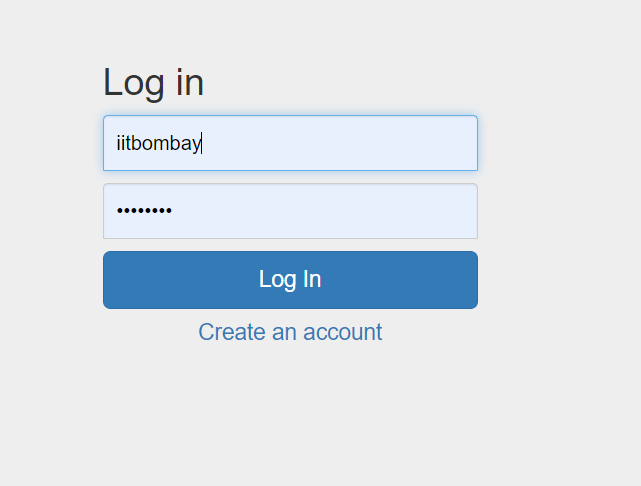
\includegraphics[width=0.5\textwidth]{images/Loginpage.PNG}
    \caption{Login Page}
\end{figure}
\item After logging in/ registering the user is redirected to the welcome page, here an API Key is given to an organization that will be used to uniquely identify the organization.
\begin{figure}[h]
    \centering
    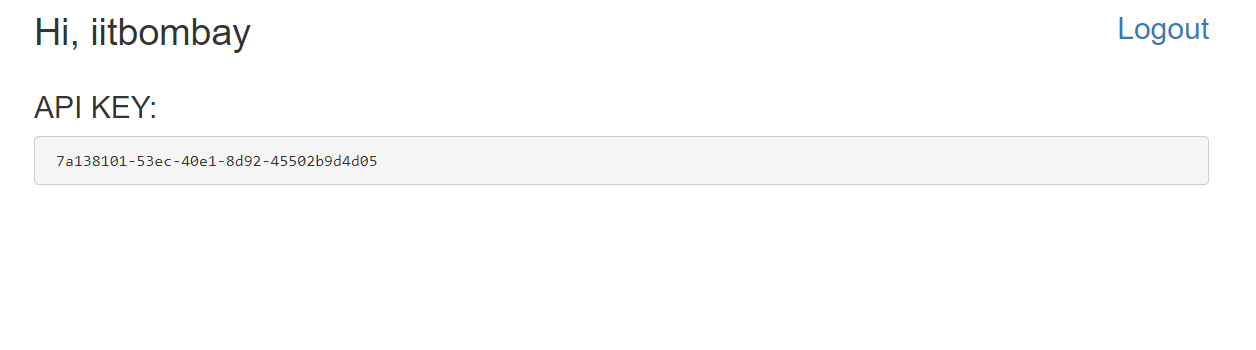
\includegraphics[width=1.0\textwidth]{WebPage.PNG}
    \caption{Welcome Page after register}
\end{figure}



\end{itemize}

\newpage
\subsection{Device registration}
\begin{itemize}
\item Now the Location Tracking Application APK should be installed in the android devices that are required to be tracked.
\begin{figure}[h]
\centering
    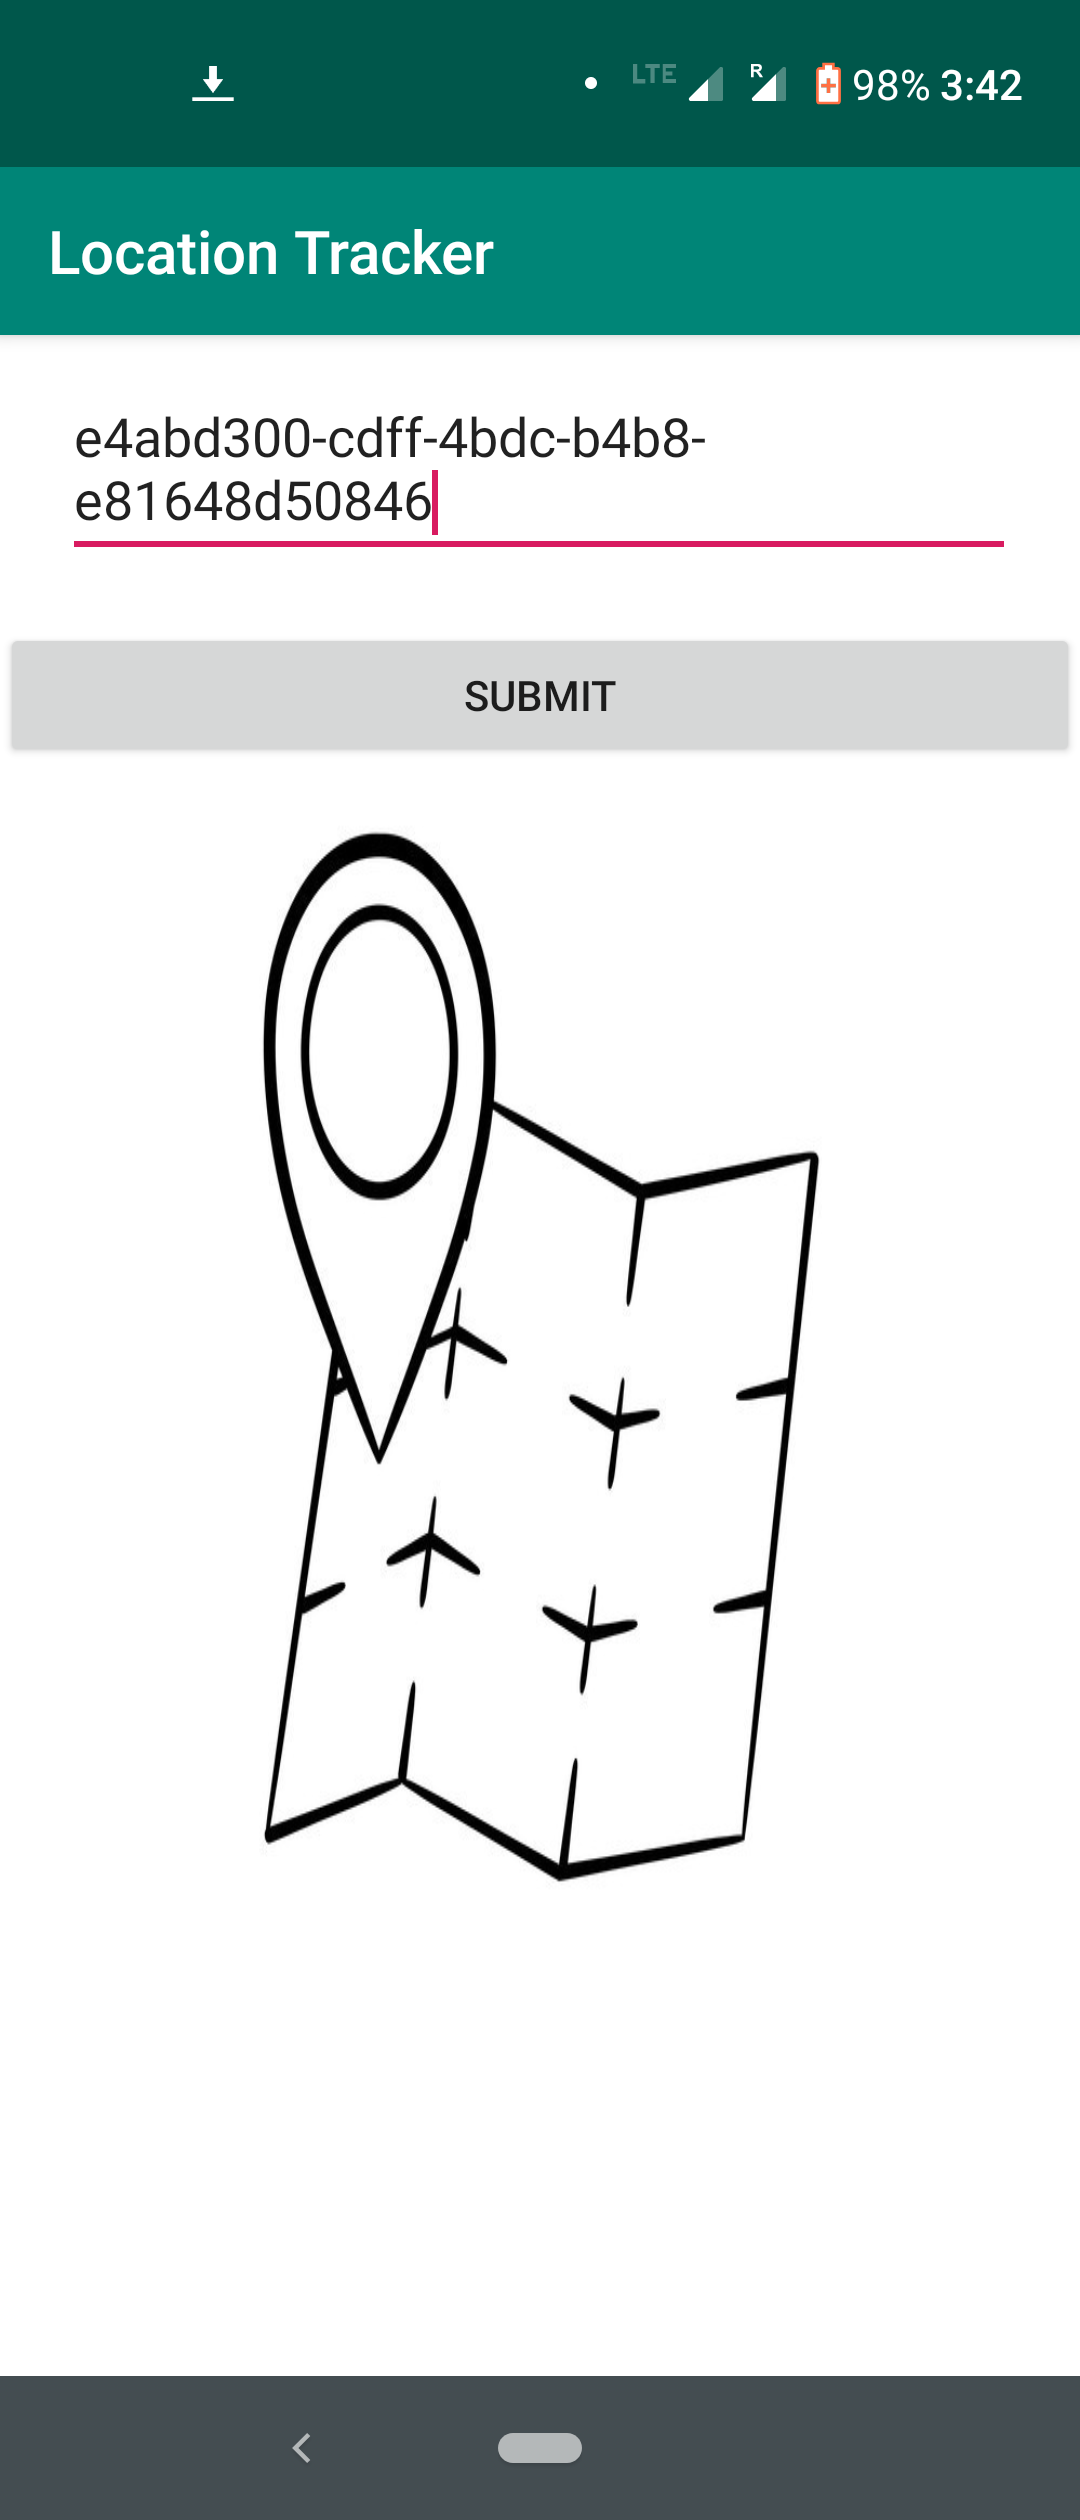
\includegraphics[width=0.25\textwidth]{images/submitAPI.png}
    \caption{Submit API key}
\end{figure}
\item When opening the application for the first time these devices needed to register with the given API key. This is a one time process as this information is stored. The device now sends the location data periodically to the server once ENABLE TRACKER is enabled.
\begin{figure}[!tbp]
  \centering
  \begin{minipage}[b]{0.4\textwidth}
  \centering
    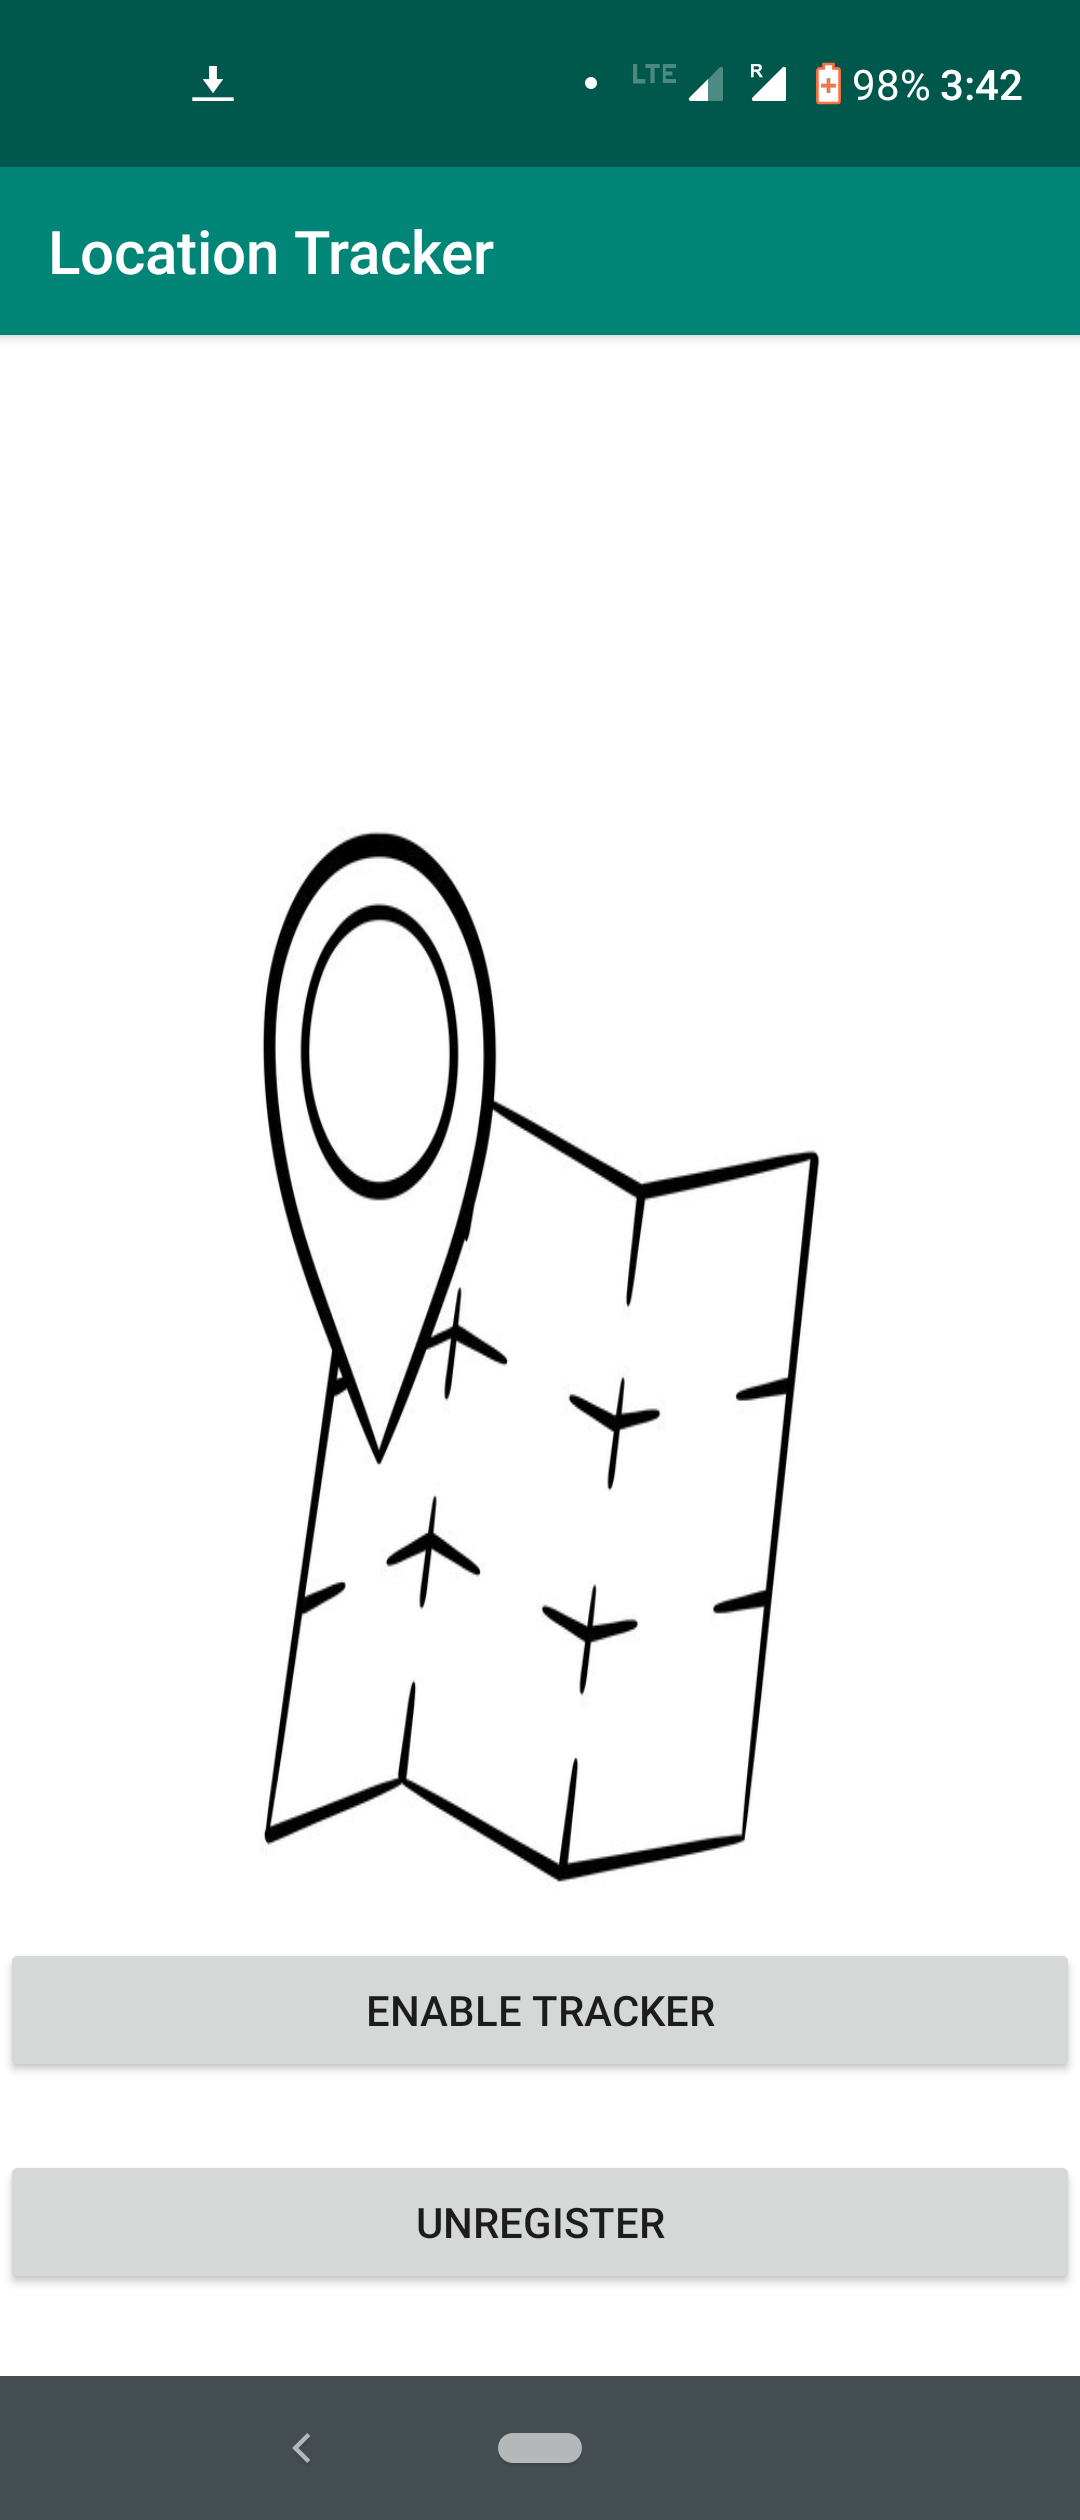
\includegraphics[width=0.6\textwidth]{images/Enabletracker.png}
    \caption{Welcome Page after register}
  \end{minipage}
  \hfill
  \begin{minipage}[b]{0.4\textwidth}
  \centering
    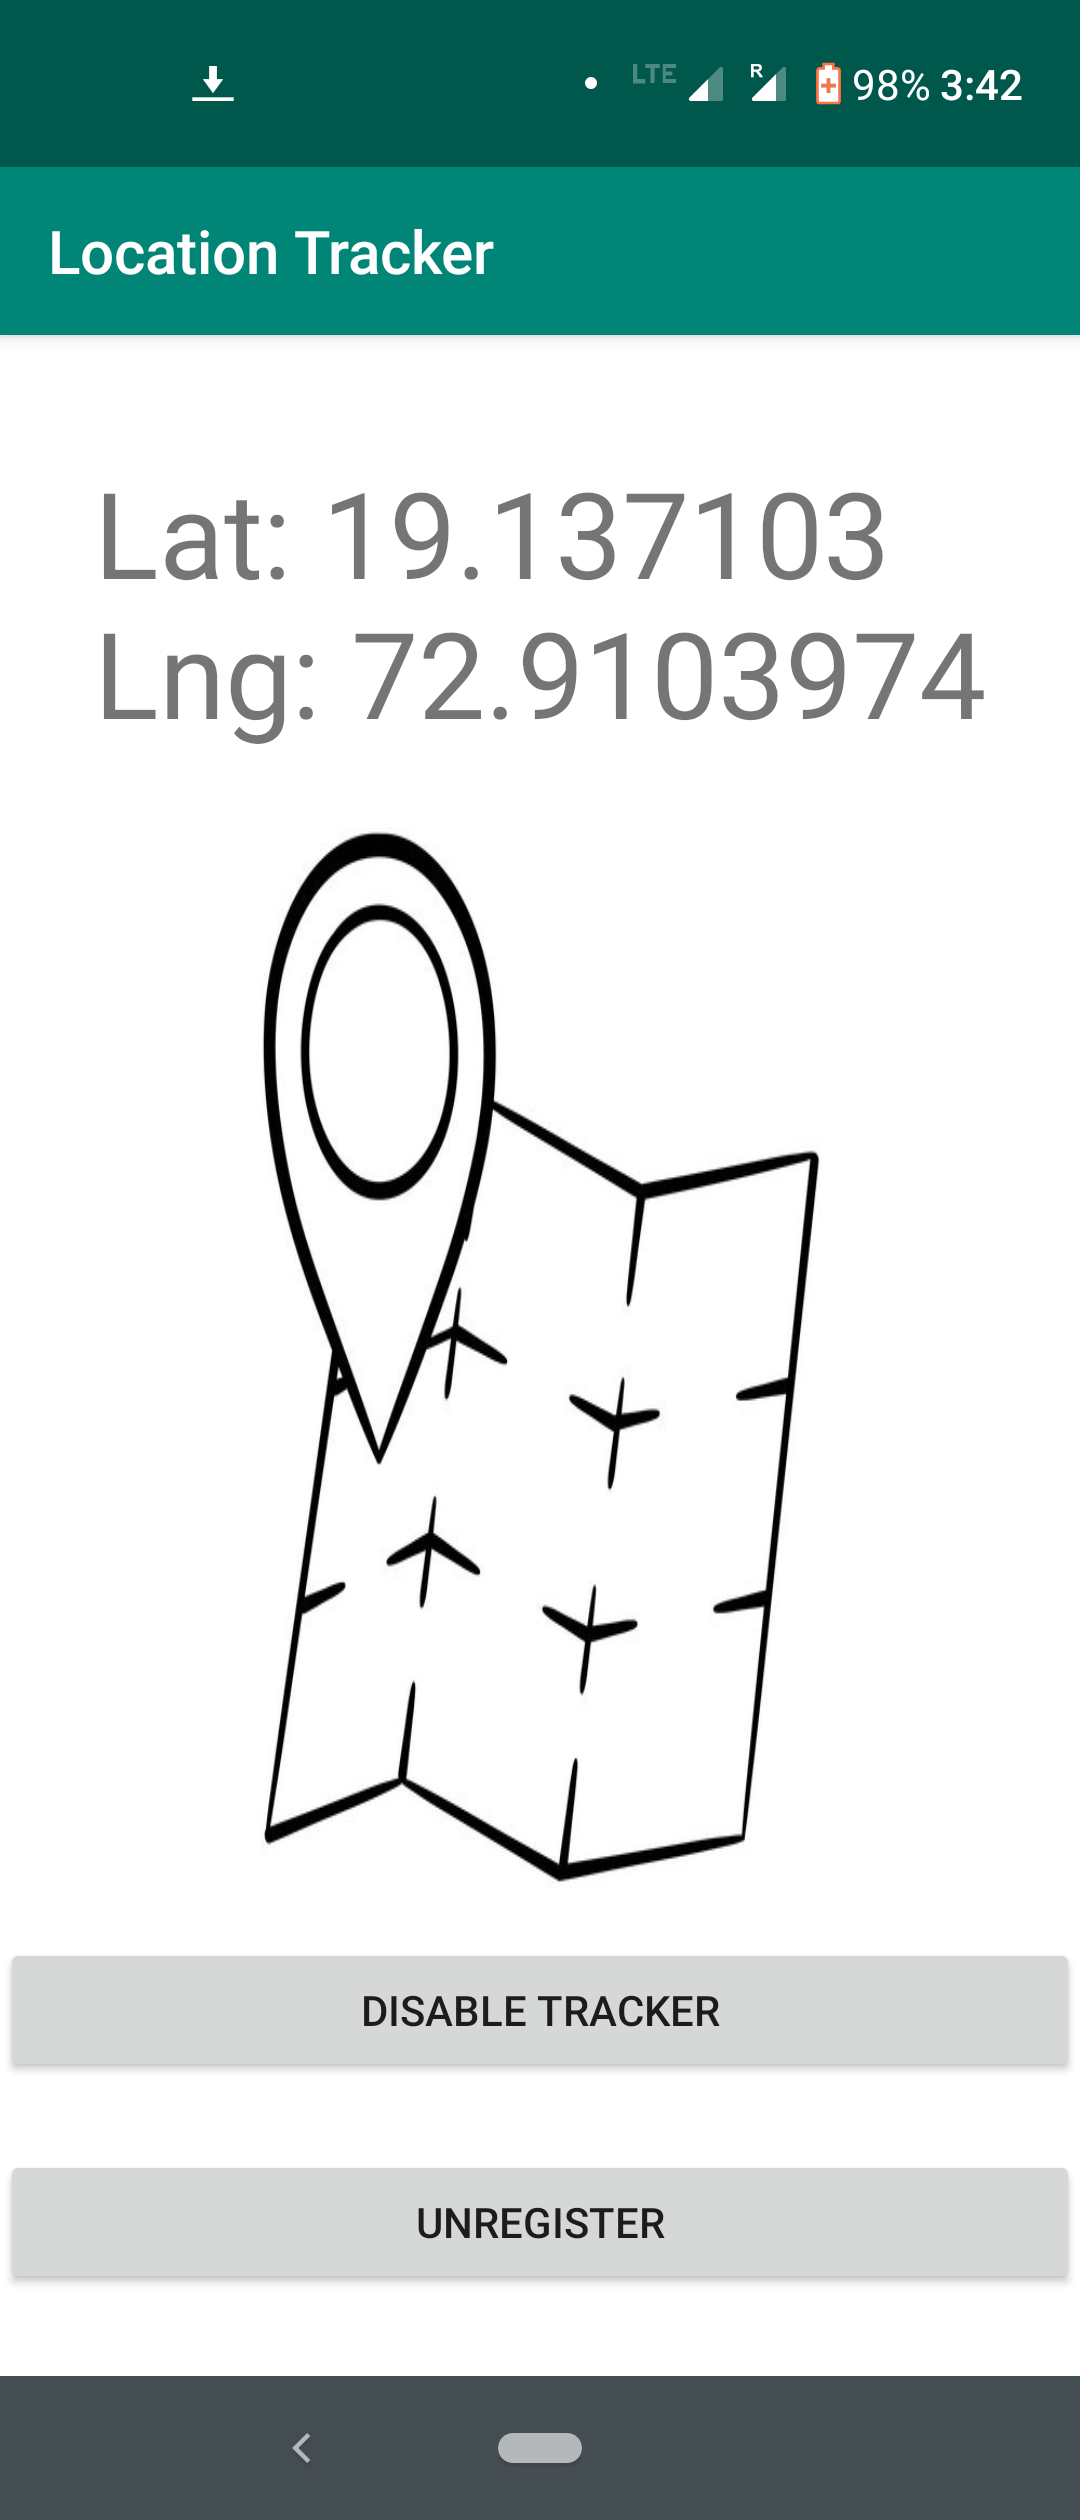
\includegraphics[width=0.6\textwidth]{images/Disabletracker.png}
    \caption{Disable Tracking / Unregister}
  \end{minipage}
\end{figure}

\end{itemize}
\newpage`

\subsection{Demo Enterprise Application}
\begin{itemize}
\item To use the location data the organization may choose to integrate out API in their own application. They may choose to show the location data on a map. 
\item This is a application where we demonstrate to implement our service to track location of E-Buggies in our campus through InstiApp.
\end{itemize}
\begin{figure}[h]
\centering
    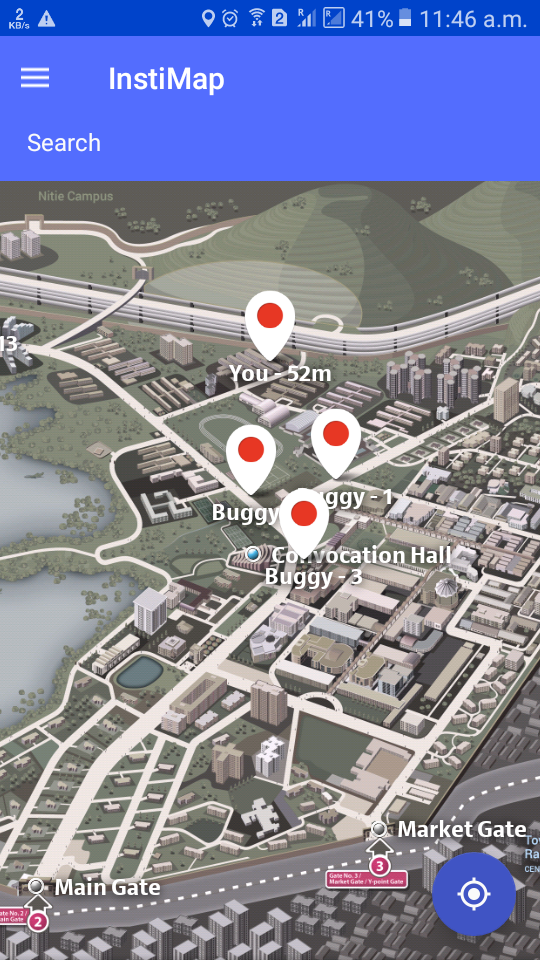
\includegraphics[width=0.25\textwidth]{images/Insti.png}
    \caption{Welcome Page after register}
\end{figure}
\newpage
Following are GET and Post requests and associated JSON object
\begin{itemize}
\item To check server status
URL: localhost:8080/api/status (GET)
\\Response:\\
\{\\
    "status": 100,\\
    "message": "Working"\\
\}
\item To register a Device
URL: localhost:8080/api/registerDevice (POST)

Request:
\{\\
"apiKey" : "SAMPLEAPIKEY",\\
"deviceId": "DEVICEID3"\\
\}

Response:
\{\\
    "status": 200,\\
    "message": "Success"\\
\}
\item To unregister a device
URL: localhost:8080/api/unregisterDevice (POST)

Request:
\{\\
"deviceId": "DEVICEID3"\\
\}

Response:
\{\\
    "status": 200,\\
    "message": "Success"\\
\}
\item Submit location from device
URL: localhost:8080/api/submitLocation (POST)

Request:
\{\\
"apiKey" : "a252fe62-faa7-461f-aecd-4cd9cae40b61",\\
"deviceId": "DEVICEID4",\\
"latLng" : \{\\
               "lat" : 100.4224764,\\
               "lng" : -122.0842499\\
            \}\\
\}

Response:
\{\\
    "status": 200,\\
    "message": "Success"\\
\}

\item Get Device Locations
URL: localhost:8080/api/getDeviceLocations (POST)

Request:
\{\\
"apiKey" : "a252fe62-faa7-461f-aecd-4cd9cae40b61"\\
\}

Response:
\{\\
    "DEVICEID1": \{\\
        "latLng": \{\\
            "lat": 100.4224764,\\
            "lng": -122.0842499\\
        \},\\
        "timestamp": "2019-11-23T13:40:53.432+0000"\\
    \},\\
    "DEVICEID2": \{\\
        "latLng": \{\\
            "lat": 100.4224764,\\
            "lng": -122.0842499\\
        \},\\
        "timestamp": "2019-11-23T13:40:48.361+0000"\\
    \},\\
    "DEVICEID3": \{\\
        "latLng": \{\\
            "lat": 100.4224764,\\
            "lng": -122.0842499\\
        \},\\
        "timestamp": "2019-11-23T13:40:42.728+0000"\\
    \},\\
    "DEVICEID4": \{\\
        "latLng": \{\\
            "lat": 100.4224764,\\
            "lng": -122.0842499\\
        \},\\
        "timestamp": "2019-11-23T13:41:11.590+0000"\\
    \}\\
\}
    
\end{itemize}
\section{Usefulness of the Project}
Our Project is built to easily integrate with existing system. We can deploy our project by having cost efficient android devices in E Buggies on our campus and our server can be deployed in college server without additional cost.The device tracking app is integrated in InstiApp Maps Section which is already working. So the only thing left is implementation in E-Buggies.
\end{document}
